% =========================================================================
% Criteri NewsGuard e regressione (Web Science 2027, tentativo 16): quali criteri NewsGuard si vedono nel testo,
% quanto pesano sul punteggio complessivo, e come si valuta un modello addestrato a prevedere il punteggio.
% Figure: figure/genera_figure.py (legge Dataset/ e Code/WebScience2027/Tentativi/16_DataPreparation).
% Build: tectonic criteri_e_regressione.tex
% =========================================================================
\documentclass[aspectratio=169]{beamer}
\usetheme{Madrid}
\usecolortheme{whale}
\usepackage[T1]{fontenc}
\usepackage{graphicx}
\usepackage{booktabs}
\usepackage{array}
\usepackage{xcolor}
\graphicspath{{./figure/}{./}}

\beamertemplatenavigationsymbolsempty
\setbeamercovered{invisible}
\newcommand{\hl}[1]{\textbf{#1}}
\newcommand{\divider}[2]{%
  \begin{frame}[plain]
    \vfill
    \begin{center}
      {\color{dividerblue}\Huge\textbf{#1}}\\[0.8em]
      {\large #2}
    \end{center}
    \vfill
  \end{frame}}
\definecolor{dividerblue}{RGB}{28,42,92}
\definecolor{testo}{RGB}{42,120,214}
\newcommand{\testo}[1]{\textcolor{testo}{\textbf{#1}}}

\title[Criteri NewsGuard e regressione]{Criteri NewsGuard e regressione}
\subtitle{Che cosa del punteggio si vede nel testo, e come valutiamo un modello che prevede il punteggio}
\author[John Bianchi]{John Bianchi}
\institute[]{IMT Lucca \& IIT-CNR Pisa}
\date{}

\begin{document}

\begin{frame}
  \titlepage
\end{frame}

% ===================================================================================================
\divider{I criteri NewsGuard}{quali si vedono negli articoli, e quanto contano}

\begin{frame}{Il punteggio NewsGuard \`e la somma di 9 criteri}
  \centering\small
  \begin{tabular}{>{\raggedright\arraybackslash}p{0.5\textwidth}r>{\raggedright\arraybackslash}p{0.26\textwidth}}
    \toprule
    \textbf{Criterio} & \textbf{Punti} & \textbf{Dove si vede} \\
    \midrule
    \testo{Non pubblica notizie false} & 22 & \testo{negli articoli} \\
    \testo{Raccoglie e presenta le informazioni con cura} & 18 & \testo{negli articoli} \\
    Corregge gli errori & 12,5 & pratica del sito \\
    \testo{Distingue notizia e opinione} & 12,5 & \testo{negli articoli} \\
    \testo{Evita i titoli ingannevoli} & 10 & \testo{negli articoli} \\
    Dichiara propriet\`a e finanziamento & 7,5 & pratica del sito \\
    Distingue la pubblicit\`a & 7,5 & pratica del sito \\
    Dice chi comanda (e i conflitti di interesse) & 5 & pratica del sito \\
    Mette i nomi degli autori & 5 & pratica del sito \\
    \bottomrule
  \end{tabular}\\[0.7em]
  \raggedright
  Ogni criterio \`e un s\`i o un no; il punteggio (0--100) \`e la somma dei punti dei s\`i. Affidabile = almeno 60.\\
  \testo{4 criteri} riguardano il contenuto (\testo{62,5 punti}); \hl{5} le pratiche e la trasparenza del sito (37,5 punti),
  che negli articoli non si vedono.
\end{frame}

\begin{frame}{Quanto ogni criterio va d'accordo con il punteggio complessivo}
  \centering
  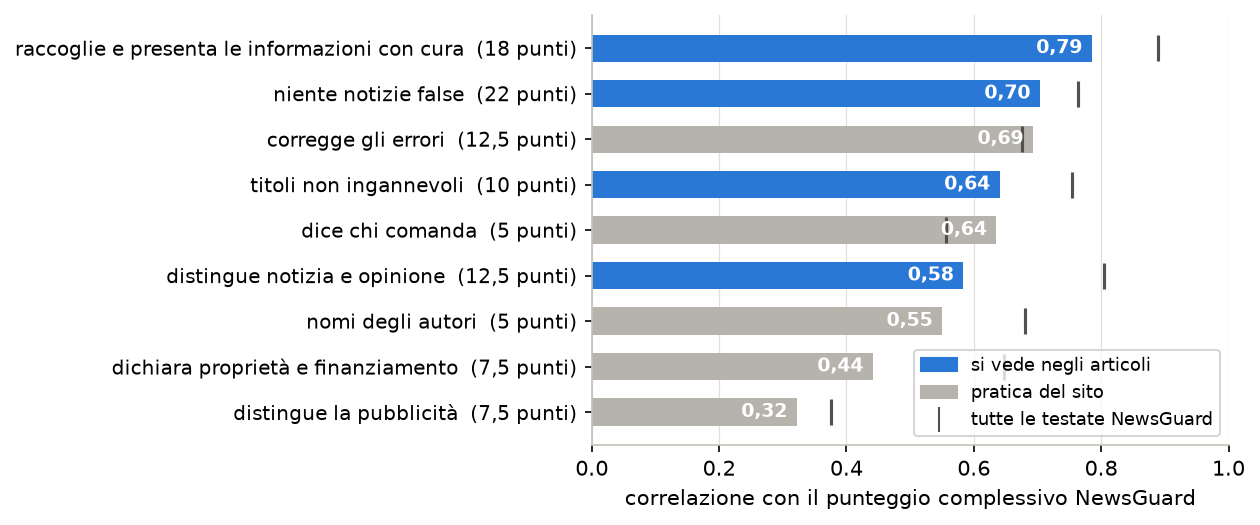
\includegraphics[width=0.92\textwidth]{correlazioni.png}\\[0.3em]
  \raggedright\small
  Barre: le nostre 226 testate (tentativo 16); trattini: tutte le 11.564 testate valutate da NewsGuard.\\
  Il criterio pi\`u legato al punteggio \`e \testo{raccoglie e presenta le informazioni con cura} (0,79; 0,89 su tutte):
  \`e il pi\`u ``testuale'' e anche il pi\`u informativo.
\end{frame}

\begin{frame}{I soli criteri sul testo spiegano quasi tutto il punteggio}
  \begin{columns}[T]
    \column{0.52\textwidth}
      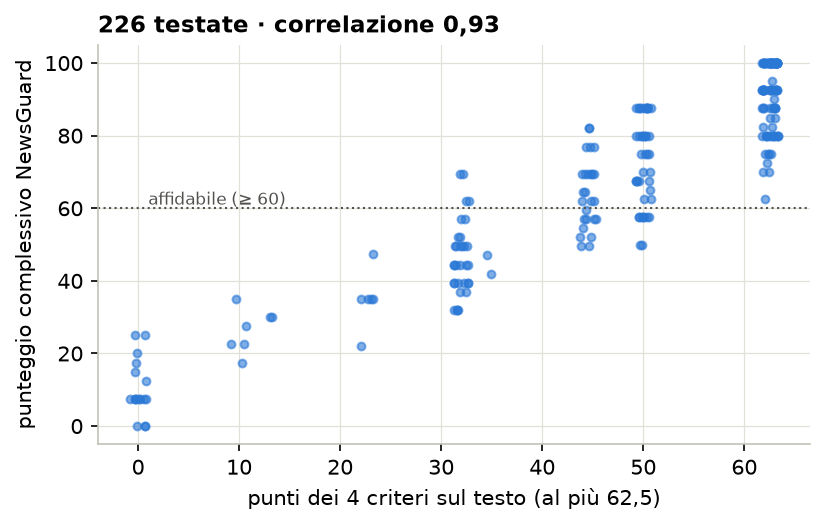
\includegraphics[width=\textwidth]{testo_e_punteggio.png}
    \column{0.46\textwidth}
      \small
      \begin{itemize}
        \setlength\itemsep{0.7em}
        \item La somma dei punti dei 4 criteri sul testo ha correlazione \hl{0,93} con il punteggio complessivo
              (0,95 su tutte le testate NewsGuard): ne spiega circa l'\hl{87\%}.
        \item Chi soddisfa tutti e 4 \`e \hl{sempre affidabile} (94 testate su 94): anche perdendo tutti i punti del sito
              resta a 62,5.
        \item Chi ne manca anche uno solo \`e inaffidabile in 79 casi su 132.
      \end{itemize}
  \end{columns}
\end{frame}

\begin{frame}{Che cosa ne segue per l'addestramento}
  \vfill
  \begin{itemize}
    \setlength\itemsep{1em}
    \item \hl{Il punteggio dei soli criteri sul testo} (0--62,5) \`e un bersaglio sensato: \`e quasi lo stesso del punteggio
          complessivo, ma toglie le pratiche del sito, che un modello che legge gli articoli non pu\`o vedere.
    \item \hl{I criteri presi uno per uno} sono pi\`u difficili: ``niente notizie false'' e ``titoli non ingannevoli''
          li soddisfa circa il 90\% delle nostre testate, quindi restano solo 23--29 esempi negativi per imparare.
    \item I criteri sono legati tra loro: misurano in buona parte la stessa cosa, la qualit\`a generale della testata.
  \end{itemize}
  \vfill
\end{frame}

% ===================================================================================================
\divider{La regressione}{come si addestra e come si valuta, passo per passo}

\begin{frame}{Passo 1 e 2: si impara un numero, la testata prende la media}
  \vfill
  \begin{enumerate}
    \setlength\itemsep{1.1em}
    \item \hl{Addestramento.} Ogni articolo eredita il punteggio NewsGuard della sua testata (da 0 a 100). Il modello
          (ridge sopra il TF-IDF o gli embedding, oppure ModernBERT) impara a prevedere quel \hl{numero}, sbagliando il meno
          possibile in media (errore quadratico).
    \item \hl{Test.} Le testate di test non sono mai state viste. Il modello d\`a un numero a ognuno dei loro articoli e la
          \hl{testata prende la media} dei numeri dei suoi articoli.
  \end{enumerate}
  \vfill
  \raggedright\small\itshape Non si misura mai la distanza esatta (``ha detto 70, era 71''): il numero si trasforma in una
  decisione, come nei passi 3 e 4.
\end{frame}

\begin{frame}{Passo 3: affidabile s\`i o no}
  \begin{columns}[T]
    \column{0.52\textwidth}
      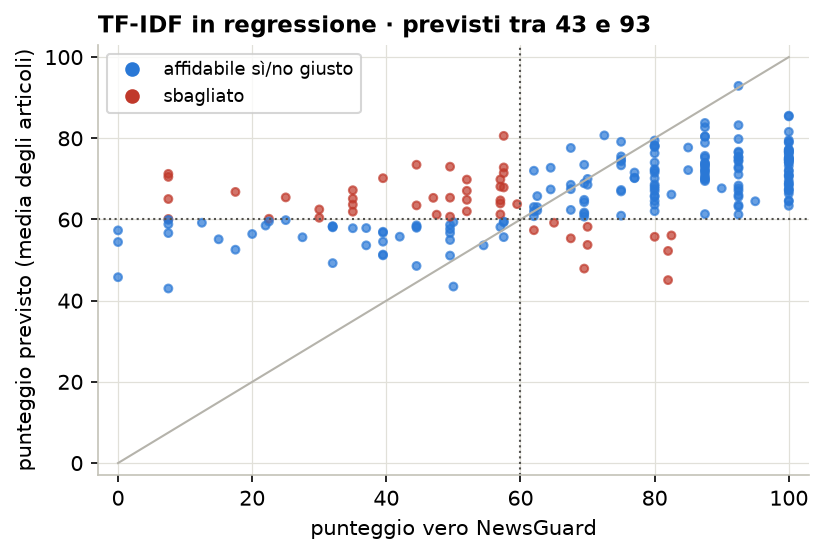
\includegraphics[width=\textwidth]{compressione.png}
    \column{0.46\textwidth}
      \small
      \begin{itemize}
        \setlength\itemsep{0.7em}
        \item Se la media prevista \`e \hl{almeno 60}, la testata \`e affidabile. \`E giusto se anche il punteggio vero \`e
              almeno 60.
        \item \hl{Previsto 70, vero 71}: tutti e due sopra 60, \hl{giusto}. Anche previsto 61 e vero 98 \`e giusto.
        \item \hl{Previsto 58, vero 61}: da una parte e dall'altra della soglia, \hl{sbagliato}, anche se la distanza \`e
              piccola.
      \end{itemize}
      \vspace{0.4em}
      In rosso le testate sbagliate (TF-IDF in regressione).
  \end{columns}
\end{frame}

\begin{frame}{Passo 4: i 5 livelli, e perch\'e non bastano le soglie di NewsGuard}
  \begin{columns}[T]
    \column{0.5\textwidth}
      \small
      \begin{itemize}
        \setlength\itemsep{0.7em}
        \item I livelli NewsGuard sono fasce di punteggio: l1 0--39, l2 40--59, l3 60--74, l4 75--99, l5 100.
        \item Ma i numeri previsti stanno \hl{stretti intorno alla media}: il TF-IDF prevede solo tra 43 e 93, mentre i veri
              vanno da 0 a 100 (nel grafico a fianco, i punti stanno su una fascia orizzontale).
        \item Con le fasce di NewsGuard nessuna testata finirebbe in \hl{l1} (sotto 40) o in \hl{l5} (100): conta di pi\`u
              l'\hl{ordine} delle testate che il numero esatto.
      \end{itemize}
    \column{0.48\textwidth}
      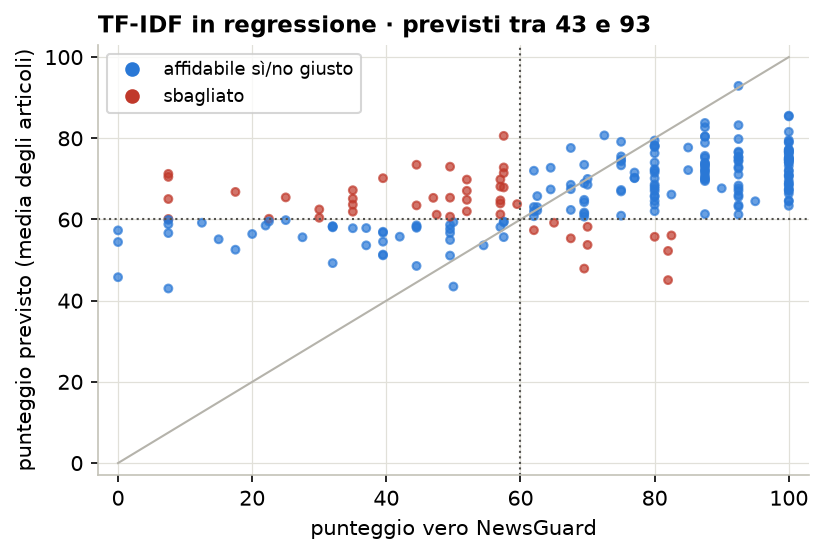
\includegraphics[width=\textwidth]{compressione.png}
  \end{columns}
\end{frame}

\begin{frame}{Passo 4: le quote del training}
  \centering
  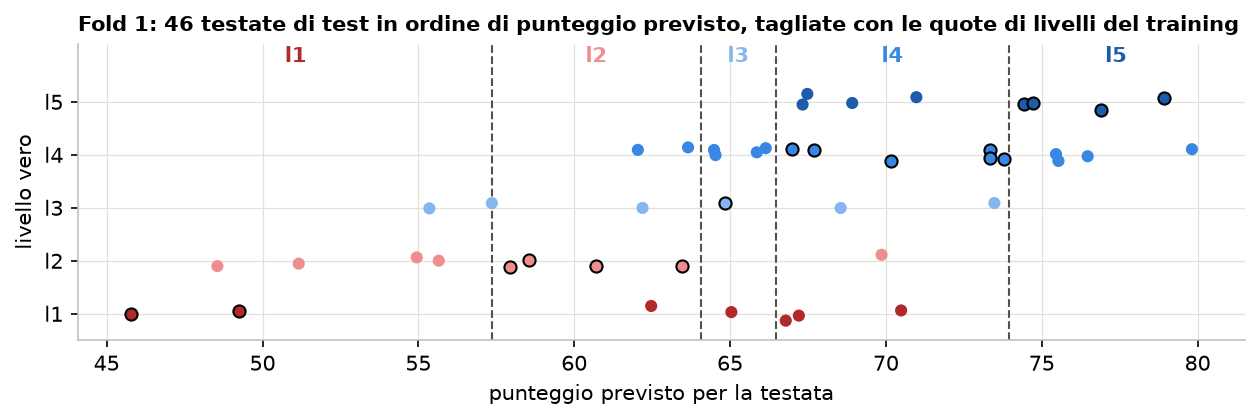
\includegraphics[width=0.93\textwidth]{quote.png}\\[0.2em]
  \raggedright\small
  Le testate di test si mettono \hl{in ordine di punteggio previsto} e si tagliano con le \hl{stesse quote di livelli del
  training} (fold 1: 16\% l1, 19\% l2, 13\% l3, 35\% l4, 17\% l5). Contorno nero = livello giusto.\\
  \hl{Previsto 70, vero 71} (l3): nel fold 1 il 70 cade in \hl{l4}, quindi per l'F1 sui 5 livelli \`e un errore, ma per la
  \hl{tolerant} ($\pm$1 livello) e per affidabile s\`i/no \`e giusto.
\end{frame}

\begin{frame}{In breve}
  \vfill
  \centering\small
  \begin{tabular}{>{\raggedright\arraybackslash}p{0.26\textwidth}>{\raggedright\arraybackslash}p{0.62\textwidth}}
    \toprule
    \textbf{Misura} & \textbf{Come si ottiene dal numero previsto per la testata} \\
    \midrule
    Affidabile s\`i/no & giusto se previsto e vero stanno dalla stessa parte di 60 \\
    \addlinespace
    F1 sui 5 livelli & testate in ordine di numero previsto, tagliate con le quote di livelli del training; giusto se il
    livello coincide \\
    \addlinespace
    Tolerant $\pm$1 & come sopra, ma \`e giusto anche un livello vicino \\
    \bottomrule
  \end{tabular}\\[1.2em]
  \raggedright
  \begin{itemize}
    \setlength\itemsep{0.6em}
    \item La distanza esatta tra previsto e vero (70 contro 71) non entra mai nelle misure: conta da che parte di 60 sta la
          testata e in che posizione sta rispetto alle altre.
    \item I classificatori a 5 classi invece danno direttamente un livello a ogni articolo, e la testata prende il
          livello votato dalla maggioranza dei suoi articoli.
  \end{itemize}
  \vfill
\end{frame}

\end{document}
